\documentclass[12pt,a4paper,oneside]{report}

% ------------------------------------------------------------------
% Page layout and typography
% ------------------------------------------------------------------
\usepackage[a4paper,left=1in,right=0.85in,top=0.9in,bottom=0.9in]{geometry}
\usepackage[T1]{fontenc}
\usepackage{tgpagella}
\usepackage[sc]{mathpazo}
\linespread{1.18}
\usepackage[final]{microtype}
\usepackage{amsmath,amssymb}
\usepackage{booktabs,tabularx,multirow,array}
\usepackage{graphicx}
\usepackage{xcolor}
\usepackage{enumitem}
\usepackage{listings}
\usepackage{caption,subcaption}
\usepackage{float}
\usepackage{titlesec}
\usepackage{fancyhdr}
\usepackage{tocloft}
\usepackage{setspace}
\usepackage[hyphens]{url}
\usepackage[hidelinks]{hyperref}
\usepackage{tikz}
\usetikzlibrary{arrows.meta,positioning,fit,calc,shapes.geometric,backgrounds}
\usepackage{pgfplots}
\pgfplotsset{compat=1.16}
\renewcommand{\topfraction}{0.85}
\renewcommand{\bottomfraction}{0.7}
\renewcommand{\textfraction}{0.15}
\renewcommand{\floatpagefraction}{0.8}
\setlength{\textfloatsep}{12pt plus 2pt minus 2pt}
\setlength{\intextsep}{10pt plus 2pt minus 2pt}

% Muted print palette
\definecolor{ink}{HTML}{222222}
\definecolor{mid}{HTML}{6B6B6B}
\definecolor{light}{HTML}{D9D9D9}
\definecolor{paper}{HTML}{F4F4F2}
\definecolor{navy}{HTML}{2F4B6E}
\definecolor{navyl}{HTML}{C9D3DF}
\definecolor{ochre}{HTML}{A8742A}
\definecolor{ochrel}{HTML}{EBDCC4}
\definecolor{rust}{HTML}{8E3B2E}

\captionsetup{font=small,labelfont=bf,labelsep=period,justification=justified,singlelinecheck=true}
\setlist{itemsep=2pt,topsep=4pt}

\titleformat{\chapter}[display]{\normalfont\bfseries\Large}{\large\scshape Chapter \thechapter}{6pt}{\LARGE}
\titlespacing*{\chapter}{0pt}{0pt}{24pt}
\titleformat{\section}{\normalfont\bfseries\large}{\thesection}{0.8em}{}
\titleformat{\subsection}{\normalfont\bfseries\normalsize}{\thesubsection}{0.8em}{}
\titleformat{\subsubsection}{\normalfont\itshape\normalsize}{\thesubsubsection}{0.8em}{}

\pagestyle{fancy}
\fancyhf{}
\fancyhead[L]{\small\itshape MPCS and LocalKG}
\fancyhead[R]{\small\itshape\nouppercase{\leftmark}}
\fancyfoot[C]{\small\thepage}
\renewcommand{\headrulewidth}{0.3pt}
\fancypagestyle{plain}{\fancyhf{}\fancyfoot[C]{\small\thepage}\renewcommand{\headrulewidth}{0pt}}

\lstset{basicstyle=\ttfamily\footnotesize,frame=lines,framerule=0.3pt,breaklines=true,
  columns=fullflexible,keepspaces=true,showstringspaces=false,
  keywordstyle=\bfseries,commentstyle=\color{mid}\itshape,language=Python,
  xleftmargin=1em,xrightmargin=1em}

\newcommand{\code}[1]{\texttt{\small #1}}
\newcommand{\ms}{\,\text{ms}}
\newcommand{\us}{\,\textmu\text{s}}

% TikZ styles
\tikzset{
  blk/.style={draw=ink,line width=0.5pt,fill=white,rounded corners=1.5pt,align=center,
              font=\footnotesize,minimum height=9mm,inner sep=4pt},
  blkn/.style={blk,fill=navyl},
  blko/.style={blk,fill=ochrel},
  blkg/.style={blk,fill=paper},
  arr/.style={-{Stealth[length=2.2mm]},line width=0.5pt,draw=ink},
  darr/.style={arr,dashed},
  grp/.style={draw=mid,dashed,line width=0.4pt,rounded corners=3pt,inner sep=6pt},
  lbl/.style={font=\scriptsize\itshape,text=mid},
}

\pgfplotsset{
  rep/.style={
    width=\linewidth,height=6.2cm,
    axis line style={ink,line width=0.4pt},
    tick style={ink,line width=0.4pt},
    tick label style={font=\footnotesize},
    label style={font=\footnotesize},
    legend style={font=\footnotesize,draw=none,fill=none},
    ymajorgrids,grid style={light,line width=0.3pt},
    axis x line*=bottom,axis y line*=left,
  }
}

\begin{document}

% ==================================================================
% Front matter
% ==================================================================
\pagenumbering{roman}
\begin{titlepage}
\centering
\vspace*{0.4cm}

\includegraphics[width=3.6cm]{figures/iitj_logo.png}\par
\vspace{1.0cm}
{\large\scshape B.Tech Project Report\par}
\vspace{1.0cm}
{\LARGE\bfseries A Memory-Perceptual Cognitive System\\[4pt] with a Grounded Clinical Knowledge Graph\par}
\vspace{0.6cm}
{\large Design, Implementation and Evaluation of MPCS and LocalKG\par}
\vspace{1.6cm}
{\large\bfseries Bachelor of Technology\\ in Computer Science and Engineering\par}
\vspace{1.4cm}
{\normalsize by\par}
\vspace{0.4cm}
\begin{tabular}{l@{\hspace{2.5em}}l}
\textbf{Aurindum Banerjee} & B23CS1006\\[2pt]
\textbf{Lokesh Motwani} & B23CS1033
\end{tabular}
\par\vspace{1.4cm}
{\normalsize Under the supervision of\par}
\vspace{0.3cm}
{\large Dr.\ Romi Banerjee\par}
\vfill
{\normalsize Department of Computer Science and Engineering\\ Indian Institute of Technology Jodhpur\par}
\vspace{0.2cm}
{\normalsize November 2026\par}
\end{titlepage}

\chapter*{Abstract}
\addcontentsline{toc}{chapter}{Abstract}
Decision support built only on large language models is hard to audit: answers are not always traceable to evidence, hard safety constraints cannot be enforced reliably, and latency is unbounded. This project builds an alternative in which decisions come from explicit, inspectable data structures and every recommendation is traceable to stored evidence.

The \emph{Memory-Perceptual Cognitive System} (MPCS) perceives four modalities as confidence-weighted categorical tuples, reacts to danger through reflex rules, retrieves similar past episodes, and adapts through reward feedback. Its retrieval path was developed in six layers: a $d$-left counting Bloom filter, a hard/soft slot filter (HyST), a modality-partitioned index (HMGI), their combination with automatic relaxation (SHMF), a near-miss guard (KERL), and time-bounded spreading activation (TIDE). \emph{LocalKG} is a typed knowledge graph of 1{,}106 nodes and 2{,}024 edges extracted from a historical materia medica and 21 PubMed records, queried by a dual-threshold engine and coupled to MPCS through a bridge module.

On a 700-record episode bank, hard-slot filtering cuts unsafe actions from 31.2\% to 1.2\%, SHMF raises clean accuracy from 34.2\% to 75.6\%, and TIDE reaches 71.9\% accuracy after reading only 2.2 of 25.4 candidates on average. A hybrid rule-plus-model extractor matches the 80.8\% keynote recall of pure model extraction with no failed batches. The integrated pipeline answers a query in about 4\ms{} on one CPU core.

\vspace{0.5em}
\noindent\textbf{Keywords:} cognitive architecture, episodic memory, counting Bloom filter, spreading activation, knowledge graph, information extraction, reinforcement from feedback, safety constraints.

\clearpage
\chapter*{Acknowledgements}
\addcontentsline{toc}{chapter}{Acknowledgements}
We are deeply grateful to our project supervisor, Dr.\ Romi Banerjee, for her guidance, encouragement and critical feedback throughout this project. Her questions shaped both the direction of the work and the way we evaluated it.

We also thank the Department of Computer Science and Engineering, Indian Institute of Technology Jodhpur, for the facilities and support provided during the course of this project.

\vspace{1.5cm}
\hfill\begin{tabular}{r}
Aurindum Banerjee (B23CS1006)\\
Lokesh Motwani (B23CS1033)
\end{tabular}

\clearpage
\tableofcontents
\clearpage

\clearpage
\pagenumbering{arabic}
\makeatletter
\renewcommand\chapter{\par\addvspace{1.6\baselineskip}\thispagestyle{fancy}\global\@topnum\z@\@afterindentfalse\secdef\@chapter\@schapter}
\makeatother
\titlespacing*{\chapter}{0pt}{0pt}{14pt}

% ==================================================================
\chapter{Introduction}
% ==================================================================
\section{Motivation}
Retrieval-augmented language models are now the default way to build question answering and decision support systems over a domain corpus. They are effective at producing fluent answers, but three properties make them a poor fit for settings where a wrong answer has a cost:
\begin{enumerate}
  \item \textbf{Traceability.} A generated answer cannot always be tied to the passage that supports it, and models are known to produce statements with no support in the retrieved context~\cite{ji2023hallucination}.
  \item \textbf{Hard constraints.} A dense similarity score cannot express that one feature must match exactly. Two situations can agree on nine of ten attributes and still require opposite actions if the tenth is the one that matters (for example, a hot versus a cold surface).
  \item \textbf{Latency.} Autoregressive generation time grows with output length and model size, so there is no fixed upper bound on how long a decision takes.
\end{enumerate}
Human cognition handles the same problem differently. Fast reflexes act before deliberation, familiar situations are recognised almost instantly, and slow reasoning is reserved for cases that are new or ambiguous~\cite{kahneman2011}. This project takes that division of labour as an engineering template.

\section{Objectives}
\begin{enumerate}
  \item Design a perception-decision-reward loop over categorical multimodal percepts with per-channel confidence.
  \item Develop and compare a sequence of memory indexing and retrieval methods, measuring accuracy, unsafe-action rate, memory footprint and latency.
  \item Construct a typed knowledge graph from a historical medical text and a set of biomedical abstracts, and compare rule-based, model-based and hybrid extraction methods.
  \item Build a query engine over the graph that can trade precision for coverage through a single parameter.
  \item Integrate the knowledge graph with the decision loop and verify the combined system with automated tests.
\end{enumerate}

\section{Scope and Disclaimer}
The knowledge source used for LocalKG is Hahnemann's \emph{Materia Medica Pura}, a historical homeopathic text. It was chosen because it is long, public domain, highly structured (remedy, body region, symptom, modifying condition) and typographically graded, which makes it a demanding test of information extraction. The clinical efficacy of homeopathy is not established by controlled evidence. Nothing in this report is a claim of therapeutic value, and the system is a research prototype rather than a medical device.

\chapter{Background}\label{ch:background}
The design draws on dual-process accounts of cognition, in which fast automatic responses precede slow deliberation~\cite{kahneman2011}; on the somatic marker view that affect biases choice~\cite{damasio1994}, represented in valence, arousal and dominance~\cite{mehrabian1996}; on spreading activation~\cite{collins1975} with ACT-R recency decay~\cite{anderson2004} and the foraging account of memory search~\cite{hills2012}; on $d$-left counting Bloom filters~\cite{bonomi2006}; and on Z-numbers for uncertain categorical values~\cite{zadeh2011}. Graph-based retrieval follows HippoRAG~\cite{gutierrez2024} and the retrieve, guard and read structure of KERL~\cite{mohbat2025}. Exact KNN and BM25~\cite{robertson2009} serve as baselines.

\chapter{System Overview}\label{ch:overview}
% ==================================================================
The system is organised as three cooperating subsystems (Figure~\ref{fig:arch}).

\begin{enumerate}
  \item \textbf{MPCS} (\code{Model/}) is the agent. It receives percepts, decides on one of five actions (\code{ignore}, \code{observe}, \code{approach}, \code{alert}, \code{withdraw}), receives a reward and stores the episode.
  \item \textbf{LocalKG} (\code{LocalKG/}) is the knowledge subsystem. It parses source texts, extracts typed entities and relations, annotates affect and weight, and answers graph queries.
  \item \textbf{The bridge} (\code{Model/experimental/09\_localrag\_bridge/}) maps a free-text query to both a graph query and an MPCS percept, and combines their outputs into one response with cited evidence.
\end{enumerate}

\begin{figure}[H]
\centering
\resizebox{0.97\linewidth}{!}{%
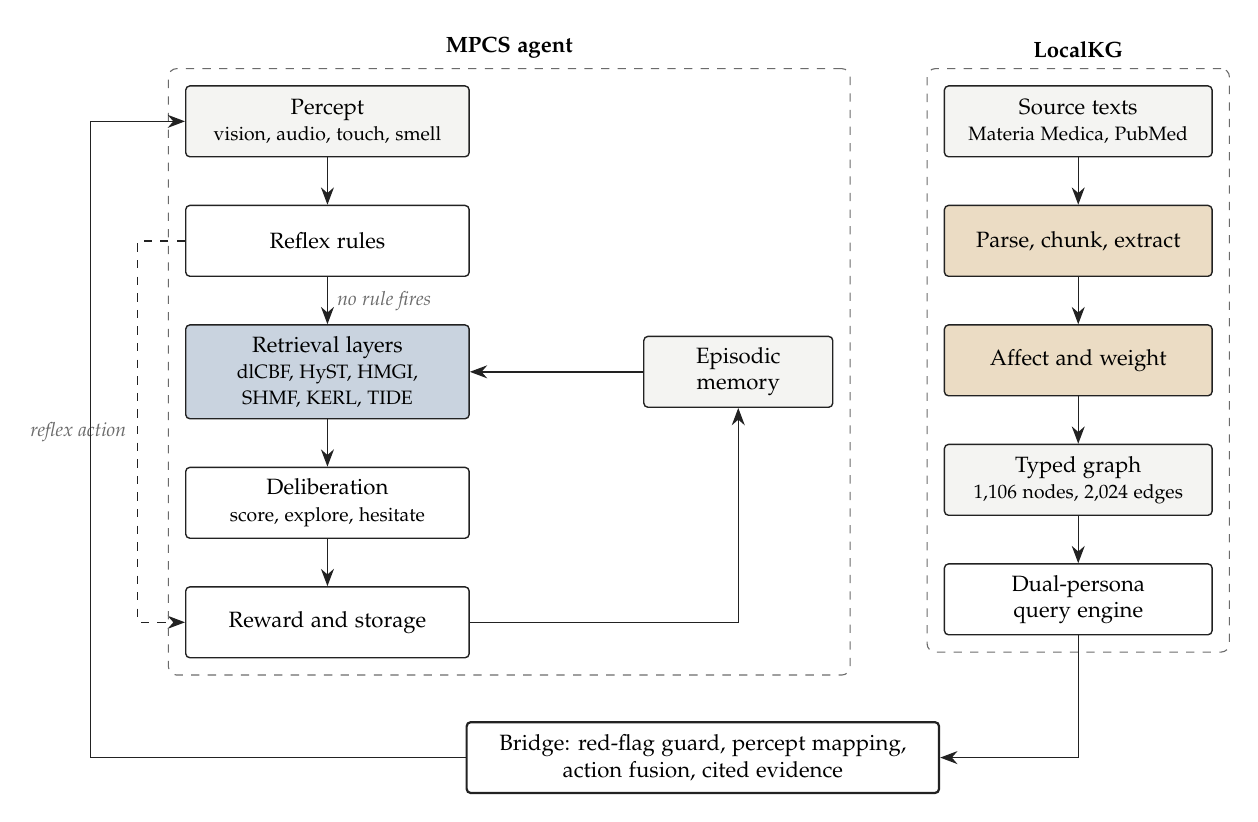
\begin{tikzpicture}[node distance=6mm and 8mm]
  % MPCS column
  \node[blkg,minimum width=36mm] (perc) {Percept\\\scriptsize vision, audio, touch, smell};
  \node[blk,below=of perc,minimum width=36mm] (refl) {Reflex rules};
  \node[blkn,below=of refl,minimum width=36mm] (ret) {Retrieval layers\\\scriptsize dlCBF, HyST, HMGI,\\\scriptsize SHMF, KERL, TIDE};
  \node[blk,below=of ret,minimum width=36mm] (dec) {Deliberation\\\scriptsize score, explore, hesitate};
  \node[blk,below=of dec,minimum width=36mm] (rew) {Reward and storage};
  \node[blkg,right=22mm of ret,minimum width=24mm] (mem) {Episodic\\memory};
  \draw[arr] (perc) -- (refl);
  \draw[arr] (refl) -- node[lbl,right]{no rule fires} (ret);
  \draw[arr] (ret) -- (dec);
  \draw[arr] (dec) -- (rew);
  \draw[arr] (mem) -- (ret);
  \draw[arr] (rew.east) -| (mem.south);
  \draw[darr] (refl.west) -- ++(-6mm,0) |- node[lbl,pos=0.25,left=3pt,fill=white,inner sep=1pt]{reflex action} (rew.west);
  \node[grp,fit=(perc)(refl)(ret)(dec)(rew)(mem),label={[font=\footnotesize\bfseries]above:MPCS agent}] (g1) {};

  % LocalKG column
  \node[blkg,minimum width=34mm,anchor=north west] (src) at ($(mem.east |- perc.north)+(14mm,0)$) {Source texts\\\scriptsize Materia Medica, PubMed};
  \node[blko,below=of src,minimum width=34mm] (ext) {Parse, chunk, extract};
  \node[blko,below=of ext,minimum width=34mm] (aff) {Affect and weight};
  \node[blkg,below=of aff,minimum width=34mm] (kg) {Typed graph\\\scriptsize 1,106 nodes, 2,024 edges};
  \node[blk,below=of kg,minimum width=34mm] (pq) {Dual-persona\\query engine};
  \draw[arr] (src) -- (ext); \draw[arr] (ext) -- (aff); \draw[arr] (aff) -- (kg); \draw[arr] (kg) -- (pq);
  \node[grp,fit=(src)(pq),label={[font=\footnotesize\bfseries]above:LocalKG}] (g2) {};

  % Bridge
  \node[blk,fill=white,line width=0.8pt,below=14mm of $(rew)!0.5!(pq)$,minimum width=60mm] (br) {Bridge: red-flag guard, percept mapping,\\ action fusion, cited evidence};
  \draw[arr] (pq.south) |- (br.east);
  \draw[arr] (br.west) -| ([xshift=-12mm]rew.south west) |- (perc.west);
\end{tikzpicture}}
\caption{Overall architecture. The MPCS agent (left) runs a perceive, decide, reward and store loop over episodic memory. LocalKG (right) builds a typed graph from source texts. The bridge (bottom) routes a query to both and merges the results.}
\label{fig:arch}
\end{figure}

\noindent The code is organised so that each retrieval generation lives in its own numbered folder (\code{04\_hyst} to \code{08\_tide}); later layers import earlier ones and no module imports a later one. This made it possible to benchmark every generation against the same memory bank in a single run.

% ==================================================================
\chapter{The MPCS Cognitive Engine}\label{ch:core}
% ==================================================================
This chapter describes the base engine in \code{Model/experimental/02\_core/mpcs\_engine.py}. All later retrieval layers reuse its percept representation, reflex rules, reward model and learning rule.

\section{Percept Representation}
A percept is a set of categorical features grouped by modality. Table~\ref{tab:modalities} lists the feature schema. Any modality can be absent; the engine reasons with whatever channels are present, and reflexes tied to a missing channel cannot fire.

\begin{table}[H]
\centering
\caption{Modalities, features and default channel confidence.}
\label{tab:modalities}
\small
\begin{tabularx}{\linewidth}{@{}l X c@{}}
\toprule
Modality & Features (values) & Conf.\\
\midrule
Vision & object type (human, animal, vehicle, unknown), motion (static, slow, fast), colour (red, blue, dark, bright) & 1.00\\
Audio & sound type (none, speech, noise, alarm), intensity (low, medium, high) & 0.90\\
Touch & contact (none, light, firm, impact), texture (smooth, rough, wet, sharp), thermal (cold, neutral, warm, hot), intensity & 0.95\\
Smell & odour type (none, food, chemical, smoke, organic), intensity (faint, moderate, strong), pleasantness & 0.70\\
\bottomrule
\end{tabularx}
\end{table}

Each feature is stored as a Z-number style pair $(v, c)$ where $c$ is the confidence of its channel. The \emph{summary} of a percept is the tuple of all such pairs, ordered by modality. Similarity between a query summary $Q$ and a stored summary $M$ is key-aligned:
\begin{equation}
  \mathrm{sim}(Q, M) = \frac{\sum_{k \in Q \cap M} \mathbb{I}[Q_k = M_k]\,\min(c^Q_k, c^M_k)}{\sum_{k \in Q} c^Q_k}.
\end{equation}
The minimum, rather than the product, of the two confidences is used so that an exact repeat scores exactly 1. Novelty is $\nu = 1 - \max_i \mathrm{sim}(Q, M_i)$ over the memory.

\section{Reflex Rules}
Seven ordered rules handle inputs that should never wait for deliberation. The first matching rule wins:
\begin{center}\small
\begin{tabular}{@{}ll@{\hspace{2em}}ll@{}}
thermal = hot & $\to$ withdraw & sound = alarm & $\to$ alert\\
contact = impact & $\to$ withdraw & sharp texture and firm contact & $\to$ withdraw\\
odour = smoke & $\to$ alert & strong chemical odour & $\to$ alert\\
motion = fast & $\to$ observe & &\\
\end{tabular}
\end{center}
The features referenced by these rules also define the default set of \emph{hard slots} used by HyST (Section~\ref{sec:hyst}).

\section{Deliberation}
When no reflex fires, every action $a$ is scored from the $k=5$ most similar memories that took $a$. Each memory $m$ contributes with weight
\begin{equation}
  w_m = \mathrm{sim}(Q, M_m)\cdot \lambda^{\,t - t_m}\cdot b_m,
\end{equation}
where $\lambda = 0.99$ is a per-step decay and $b_m$ is a boost of $3.0$ for expert-taught memories (and $2.0$ for reflex-origin memories on the reflex path). The score of $a$ is the weighted mean reward $\bar r_a$ and its \emph{support} is $\sum w_m$. Only actions with non-zero support are eligible; with no evidence the engine falls back to \code{observe}.

Exploration uses an $\varepsilon$-greedy policy whose rate grows with novelty:
\begin{equation}
  \varepsilon = \mathrm{clip}_{[0,1]}\big(\rho\,(0.6 + 0.4\,\nu)\big),
\end{equation}
where $\rho$ is the risk bias of the active profile (0.20 cautious, 0.50 balanced, 0.82 exploratory). If the exploited action scores below the current action threshold $\tau$, the engine \emph{hesitates} and takes \code{observe} instead.

\section{Reward and Learning}
\paragraph{Reward from memory.} The reward for an action is drawn around the mean of relevant past rewards, $r \sim \mathcal{N}(\bar r_a, 0.08^2)$, clipped to $[0,1]$. With no relevant memory a weak neutral prior $\mathcal{U}(0.4, 0.6)$ is used and the response is labelled as cold-start.

\paragraph{Off-recommendation penalty.} If the action taken differs from the best-evidenced action $a^*$, the reward is reduced in proportion to how much better $a^*$ looked and how well supported it was:
\begin{equation}
  p = \mathrm{clip}\Big((\bar r_{a^*} - \bar r_a)\cdot \min\big(1, \tfrac{S_{a^*}}{2.0}\big)\Big), \qquad r' = \max\big(0.10,\; r(1-p)\big).
\end{equation}
A marginally worse choice is barely penalised; overriding a strong, well-supported recommendation is.

\paragraph{Threshold adaptation.} After each step the action threshold moves with the reward, and moves further in novel situations:
\begin{equation}
  \tau \leftarrow \mathrm{clip}_{[0,1]}\big(\tau + \eta\,(0.5 + \nu)(r - 0.5)\big), \qquad \eta = 0.01.
\end{equation}
Users can also correct a decision: \code{apply\_reward} overwrites the stored reward, and \code{teach\_expert} stores the correct action as an expert memory with reward $0.95$ and boost $3.0$.

\section{Memory Banks}
Three preset banks are used. Bank~v2 contains 70 hand-designed experiences and is used for interactive work and the bridge. Bank~v3 contains 700 canonical records generated from archetype scenes, and is used with 480 clean archetype queries and 480 perturbed (noisy) queries for all benchmarks in Chapter~\ref{ch:results}.

% ==================================================================
\chapter{Memory Indexing and Retrieval Layers}\label{ch:index}
% ==================================================================
Linear scanning of memory with soft similarity has two problems: its cost grows with the store, and it can rank a memory highly even when it disagrees on a feature that determines safety. The six layers below address these issues in turn. Figure~\ref{fig:cascade} shows how they compose at query time.

\begin{figure}[H]
\centering
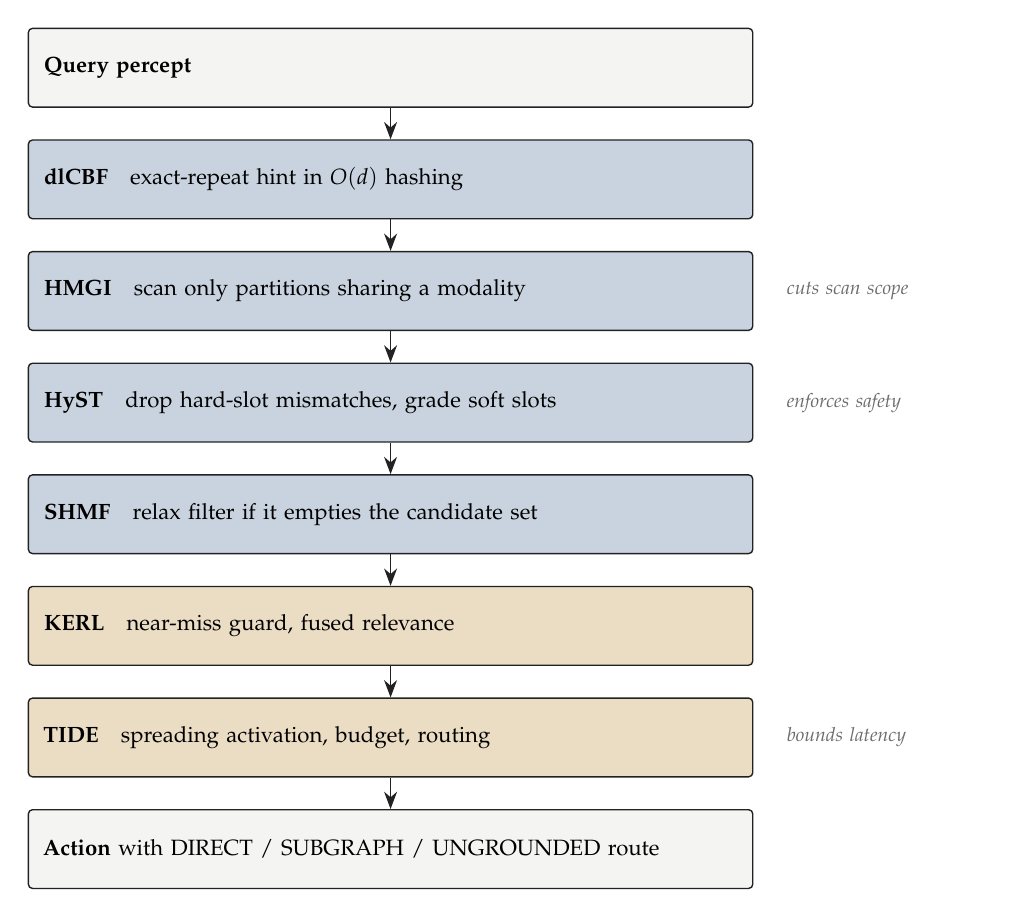
\begin{tikzpicture}[node distance=4mm]
  \tikzset{st/.style={blk,minimum width=92mm,minimum height=10mm,text width=88mm,align=left}}
  \node[st,fill=paper] (q) {\textbf{Query percept}};
  \node[st,fill=navyl,below=of q] (l1) {\textbf{dlCBF}\quad exact-repeat hint in $O(d)$ hashing};
  \node[st,fill=navyl,below=of l1] (l2) {\textbf{HMGI}\quad scan only partitions sharing a modality};
  \node[st,fill=navyl,below=of l2] (l3) {\textbf{HyST}\quad drop hard-slot mismatches, grade soft slots};
  \node[st,fill=navyl,below=of l3] (l4) {\textbf{SHMF}\quad relax filter if it empties the candidate set};
  \node[st,fill=ochrel,below=of l4] (l5) {\textbf{KERL}\quad near-miss guard, fused relevance};
  \node[st,fill=ochrel,below=of l5] (l6) {\textbf{TIDE}\quad spreading activation, budget, routing};
  \node[st,fill=paper,below=of l6] (o) {\textbf{Action} with DIRECT / SUBGRAPH / UNGROUNDED route};
  \foreach \a/\b in {q/l1,l1/l2,l2/l3,l3/l4,l4/l5,l5/l6,l6/o} \draw[arr] (\a)--(\b);
  \node[lbl,right=3mm of l2,text width=26mm] {cuts scan scope};
  \node[lbl,right=3mm of l3,text width=26mm] {enforces safety};
  \node[lbl,right=3mm of l6,text width=26mm] {bounds latency};
\end{tikzpicture}
\caption{The retrieval cascade. Shaded blue layers reduce or filter the candidate set; ochre layers decide how the surviving candidates are read.}
\label{fig:cascade}
\end{figure}

\section{Layer 1: $d$-Left Counting Bloom Filter}
The filter has $d = 4$ subtables of $1{,}024$ buckets each and stores 16-bit fingerprints with a counter. A percept summary is serialised and hashed with BLAKE2b (32-byte digest). The fingerprint is the first eight bytes masked to 16 bits (replaced by 1 if zero, so that 0 can mark an empty bucket), and the bucket index in subtable $j$ is bytes $8+4j$ to $12+4j$ modulo $1{,}024$. On insertion, an existing bucket with a matching fingerprint is incremented; otherwise the item goes to the least-loaded candidate bucket, with ties broken towards the leftmost subtable. Queries and deletions inspect the same four buckets.

On Bank~v3 the filter occupies 8.8\,KB (12.8 bytes per record) and answers a query in 0.017\ms{} on average. Because it only recognises exact repeats, it rejects 61.9\% of clean and 85.4\% of noisy queries. It is therefore used as a constant-time ``seen before'' hint rather than a gate that blocks retrieval.

\section{Layer 2: HyST Hard/Soft Slot Filter}\label{sec:hyst}
HyST (\code{04\_hyst/hyst\_layer.py}) splits features into hard and soft slots through a \code{SlotPolicy} object. The default hard slots are the features used by the reflex rules (thermal, contact, texture, sound type, odour type, odour intensity and motion). A memory survives only if it agrees with the query on every hard slot the query specifies:
\begin{equation}
  \mathrm{admit}(M, Q) = \prod_{k \in H \cap \mathrm{dom}(Q)} \mathbb{I}\left[M_k = Q_k\right].
\end{equation}
Survivors are ranked by a soft kernel. For ordinal features (for example thermal or intensity), partial credit is given by distance on the scale:
\begin{equation}
  K(v_a, v_b) = \max\Big(0,\; 1 - \frac{|\mathrm{idx}(v_a) - \mathrm{idx}(v_b)|}{L - 1}\Big),
\end{equation}
where $L$ is the number of levels. Two run-time modes change the behaviour: \code{urgent} keeps hard constraints absolute and returns only the nearest neighbour, while \code{divergent} turns each hard mismatch into a multiplicative discount of $0.6$ instead of an exclusion, allowing analogical retrieval.

\section{Layer 3: HMGI Modality-Partitioned Index}
HMGI (\code{05\_hmgi}) gives every stored episode a relational facet: typed edges to the previous episode and to episodes sharing the same action or object. It also buckets records by their set of active modalities, so a query scans only partitions that share at least one modality with it. On its own, HMGI changes scan scope but not ranking, so its accuracy equals that of the base engine (Table~\ref{tab:master}).

\section{Layer 4: SHMF Combined Filter}
SHMF (\code{06\_shmf}) runs HMGI first and HyST on the reduced set. This order is exact rather than approximate: a record dropped by HMGI shares no modality with the query, so HyST would have given it no hard-slot evidence and a zero soft score. The module includes a check that verifies this equivalence on a live bank. When the strict filter leaves no candidates (18.3\% of clean queries under HyST alone), SHMF repeats the search with relaxed constraints instead of returning nothing.

\section{Layer 5: KERL Guard and Fused Relevance}
KERL (\code{07\_kerl}) adapts the retrieve, guard and read structure of Mohbat and Zaki~\cite{mohbat2025}. A \emph{near-miss guard} admits a relaxed candidate only if its recorded modalities cover the channels of the query's hard slots, which prevents, for example, an audio-only memory from deciding a thermal case. Each admitted candidate gets a fused relevance
\begin{equation}
  R(m) = w_s\,\mathrm{sim}_{\text{sem}} + w_e\,\mathrm{sim}_{\text{aff}} + w_g\,g(m), \qquad (w_s, w_e, w_g) = (0.7, 0.15, 0.3),
\end{equation}
where $g(m)$ is a two-hop graph term over episode edges and the affect weight $w_e$ is active only when affect is enabled. Three heads read the candidate set: action values with support, an affect estimate, and a plain-language explanation. When nothing is admissible the step is labelled \code{UNGROUNDED} and falls back to \code{observe}.

\section{Layer 6: TIDE Time-Bounded Spreading Activation}\label{sec:tide}
TIDE (\code{08\_tide/tide\_layer.py}) keeps KERL's retrieval and changes how the retrieved structure is read.

\paragraph{Seeding.} Each admitted candidate $i$ receives initial activation
\begin{equation}
  A_i^{(0)} = \mathrm{sim}(Q, M_i)\,(1 + \beta\,a_i)\,b_i, \qquad \beta = 0.8,
\end{equation}
where $a_i$ is the arousal of the remembered episode and $b_i$ the expert or reflex boost. Seeds below $5\%$ of the strongest seed are pruned.

\paragraph{Propagation.} Activation spreads for $H = 3$ hops over typed edges with weights $w_{\text{object}} = w_{\text{place}} = 1.0$, $w_{\text{action}} = 0.7$, $w_{\text{prev}} = 0.5$:
\begin{equation}
  A_j^{(h+1)} = A_j^{(h)} + \sum_{i \in \mathcal{N}(j)} \frac{\gamma\, A_i^{(h)}}{|\mathcal{N}(i)|}\, w_{\tau(i,j)}\,(1 + \Delta t_j)^{-0.2},
\end{equation}
with hop decay $\gamma = 0.5$, out-degree normalisation and an ACT-R style recency factor~\cite{anderson2004}. At most 80 nodes remain active. Percepts may also carry a place (for example \code{kitchen/stove}); episodes at the same place are linked and receive a relevance bonus proportional to the shared path prefix.

\paragraph{Sufficiency routing.} If the best action leads the runner-up by at least $0.25$ with support of at least $0.8$, the output is \code{DIRECT} (action and a one-line reason). Otherwise it is \code{SUBGRAPH}, and the activated structure is returned for inspection. With no evidence it is \code{UNGROUNDED}.

\paragraph{Anytime mode.} Under the \code{urgent} flag, candidates are read in decreasing order of activation and reading stops after a budget of $B$ candidates (or a wall-clock deadline, 2\ms{} by default). The decision is made on what has been read. A \emph{passive} pass then reads all candidates, in a background thread, and records whether it agrees with the fast decision.

% ==================================================================
\chapter{LocalKG: Knowledge Graph Construction}\label{ch:kg}
% ==================================================================
\section{Sources}
The primary source is Hahnemann's \emph{Materia Medica Pura}~\cite{hahnemann1880}, processed for 30 remedies, with Boericke's \emph{Pocket Manual}~\cite{boericke1927} used for the extraction comparison. In addition, 21 PubMed abstracts covering 12 remedies were collected (\code{docs/Materia\_Medica\_PubMed\_Records.json}) and attached as a separate, explicitly labelled section so that historical and modern sources are never mixed.

\section{Ontology}
The schema (\code{LocalKG/src/lkg/schema/graph.py}) defines nine entity types and twelve relation types. Table~\ref{tab:ontology} shows the entity types with their counts in the final graph. The Etiology type is defined but not yet populated.

\begin{table}[H]
\centering
\caption{Entity types of the LocalKG ontology and counts in the final graph.}
\label{tab:ontology}
\small
\begin{tabularx}{\linewidth}{@{}l X r@{}}
\toprule
Entity type & Description & Nodes\\
\midrule
Medicine & Remedy (botanical, mineral or animal source) & 41\\
Physical Symptom & Somatic finding, linked to a body region & 623\\
Affective Symptom & Mental or emotional finding, annotated with VAD & 195\\
Modality & Condition that worsens or improves a symptom & 128\\
Clinical Condition & Named condition (from PubMed and text) & 79\\
Sensation & Quality of a sensation (burning, tearing, \ldots) & 20\\
Body Region & Anatomical region & 14\\
Cognitive Domain & Grouping of affective symptoms & 6\\
Etiology & Precipitating cause & 0\\
\midrule
Total & & 1{,}106\\
\bottomrule
\end{tabularx}
\end{table}

\section{Ingestion Pipeline}
Figure~\ref{fig:extract} shows the pipeline. Pages are parsed into remedy and section blocks (\code{ingest/parse\_pdf.py}) and chunked at section boundaries. A cleaning step (\code{clean\_ocr\_text} in \code{extract/affect.py}) removes prover timing annotations such as ``(aft. 6 h.)'', rejoins words split by line-end hyphens, corrects frequent OCR substitutions and strips replacement characters. Each chunk is then passed to the extractor, whose output is validated against a Pydantic schema; every extracted symptom must carry an evidence quote that is an exact substring of the chunk. Model responses are cached on disk by content hash (\code{data/llm\_cache/}) so that rebuilding the graph is deterministic. Duplicate entities are merged through alias tables and normalisation (\code{resolve/}).

\begin{figure}[H]
\centering
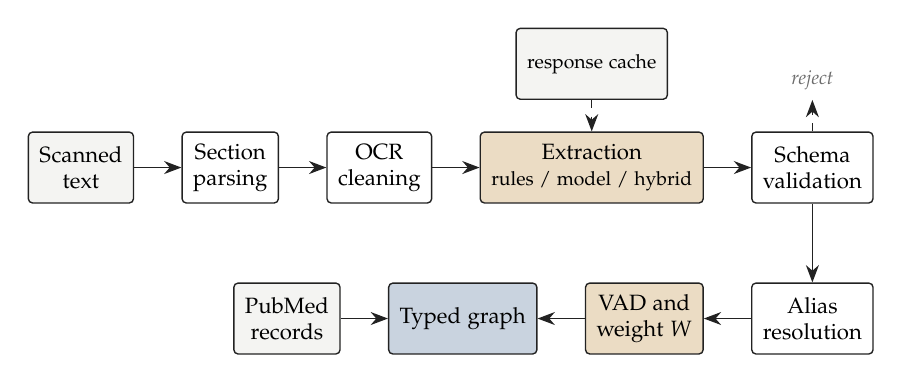
\begin{tikzpicture}[node distance=5mm and 6mm]
  \node[blkg] (a) {Scanned\\text};
  \node[blk,right=of a] (b) {Section\\parsing};
  \node[blk,right=of b] (c) {OCR\\cleaning};
  \node[blko,right=of c] (d) {Extraction\\\scriptsize rules / model / hybrid};
  \node[blk,right=of d] (e) {Schema\\validation};
  \node[blk,below=10mm of e] (f) {Alias\\resolution};
  \node[blko,left=of f] (g) {VAD and\\weight $W$};
  \node[blkn,left=of g] (h) {Typed graph};
  \node[blkg,left=of h] (i) {PubMed\\records};
  \node[blkg,above=4mm of d,font=\scriptsize] (cache) {response cache};
  \foreach \x/\y in {a/b,b/c,c/d,d/e,e/f,f/g,g/h} \draw[arr] (\x)--(\y);
  \draw[arr] (i)--(h);
  \draw[darr] (cache)--(d);
  \draw[darr] (e.north) -- ++(0,4mm) node[lbl,above]{reject};
\end{tikzpicture}
\caption{LocalKG ingestion pipeline. Validated extractions are merged, annotated with affect and weight, and combined with PubMed-derived nodes.}
\label{fig:extract}
\end{figure}

\section{Comparison of Extraction Methods}\label{sec:extraction}
Three extractors were implemented in \code{Extraction\_KRAG/homeopathy-kg} and evaluated against a gold set of 26 keynote symptoms over 8 remedies:
\begin{enumerate}
  \item \textbf{Rule-based.} Regular expressions and punctuation splitting. Fully offline and always faithful to the text, but it produces many non-symptom fragments and depends heavily on section headings.
  \item \textbf{Model-only.} An open-weights 120B-parameter language model (\code{gpt-oss-120b}) prompted to emit JSON matching the schema. It understands archaic phrasing well but 24 chunks (21\%) failed schema validation because of truncated output, timeouts or null fields.
  \item \textbf{Hybrid.} The rule-based stage proposes candidates that are grounded verbatim in the chunk; the model then audits them, removing noise and correcting their type. If the audit fails, the rule-based candidates are kept, so a batch can never fail.
\end{enumerate}

\begin{table}[H]
\centering
\caption{Extraction methods on the keynote gold set (8 remedies, 26 keynotes).}
\label{tab:extract}
\small
\begin{tabular}{@{}lrrrrr@{}}
\toprule
Method & Recall & Precision & F1 & Symptoms & Failed chunks\\
\midrule
Rule-based & 61.5\% & 4.0\% & 7.5\% & 401 & 0\\
Model-only & 80.8\% & 4.9\% & 9.2\% & 432 & 24 (21\%)\\
Hybrid & 80.8\% & 5.4\% & 10.1\% & 388 & 0\\
\bottomrule
\end{tabular}
\end{table}

Precision is low for every method because the gold set lists only keynotes, while the extractors correctly return all symptoms in a chunk; precision here should be read as a relative measure. The hybrid method keeps the recall of the model-only method, produces fewer symptoms (because noise is removed), and has no failed chunks. Three typical errors that the audit corrects are: an abbreviation (``St. Ignatius Bean'') split at the period into a symptom named ``St''; a substance name (``Common Salt'') extracted as a symptom; and ``grief'' typed as a physical symptom because it appeared in an introduction rather than a Mind section.

\section{Affect, Weighting and Graph}
Affective symptoms are annotated with VAD coordinates from a cue lexicon and grouped into six cognitive domains. Each symptom receives a weight $W = 3\cdot\mathrm{clip}(0.40\,G/3 + 0.30\,S + 0.20\,A + 0.10\,C)$ from its typographic grade $G$, adjective severity $S$, arousal $A$ and extraction confidence $C$. Modality lines produce \code{AGGRAVATED\_BY} and \code{AMELIORATED\_BY} edges. The final graph has 1,106 nodes and 2,024 edges (Figure~\ref{fig:kgfull}).

\begin{figure}[H]
\centering
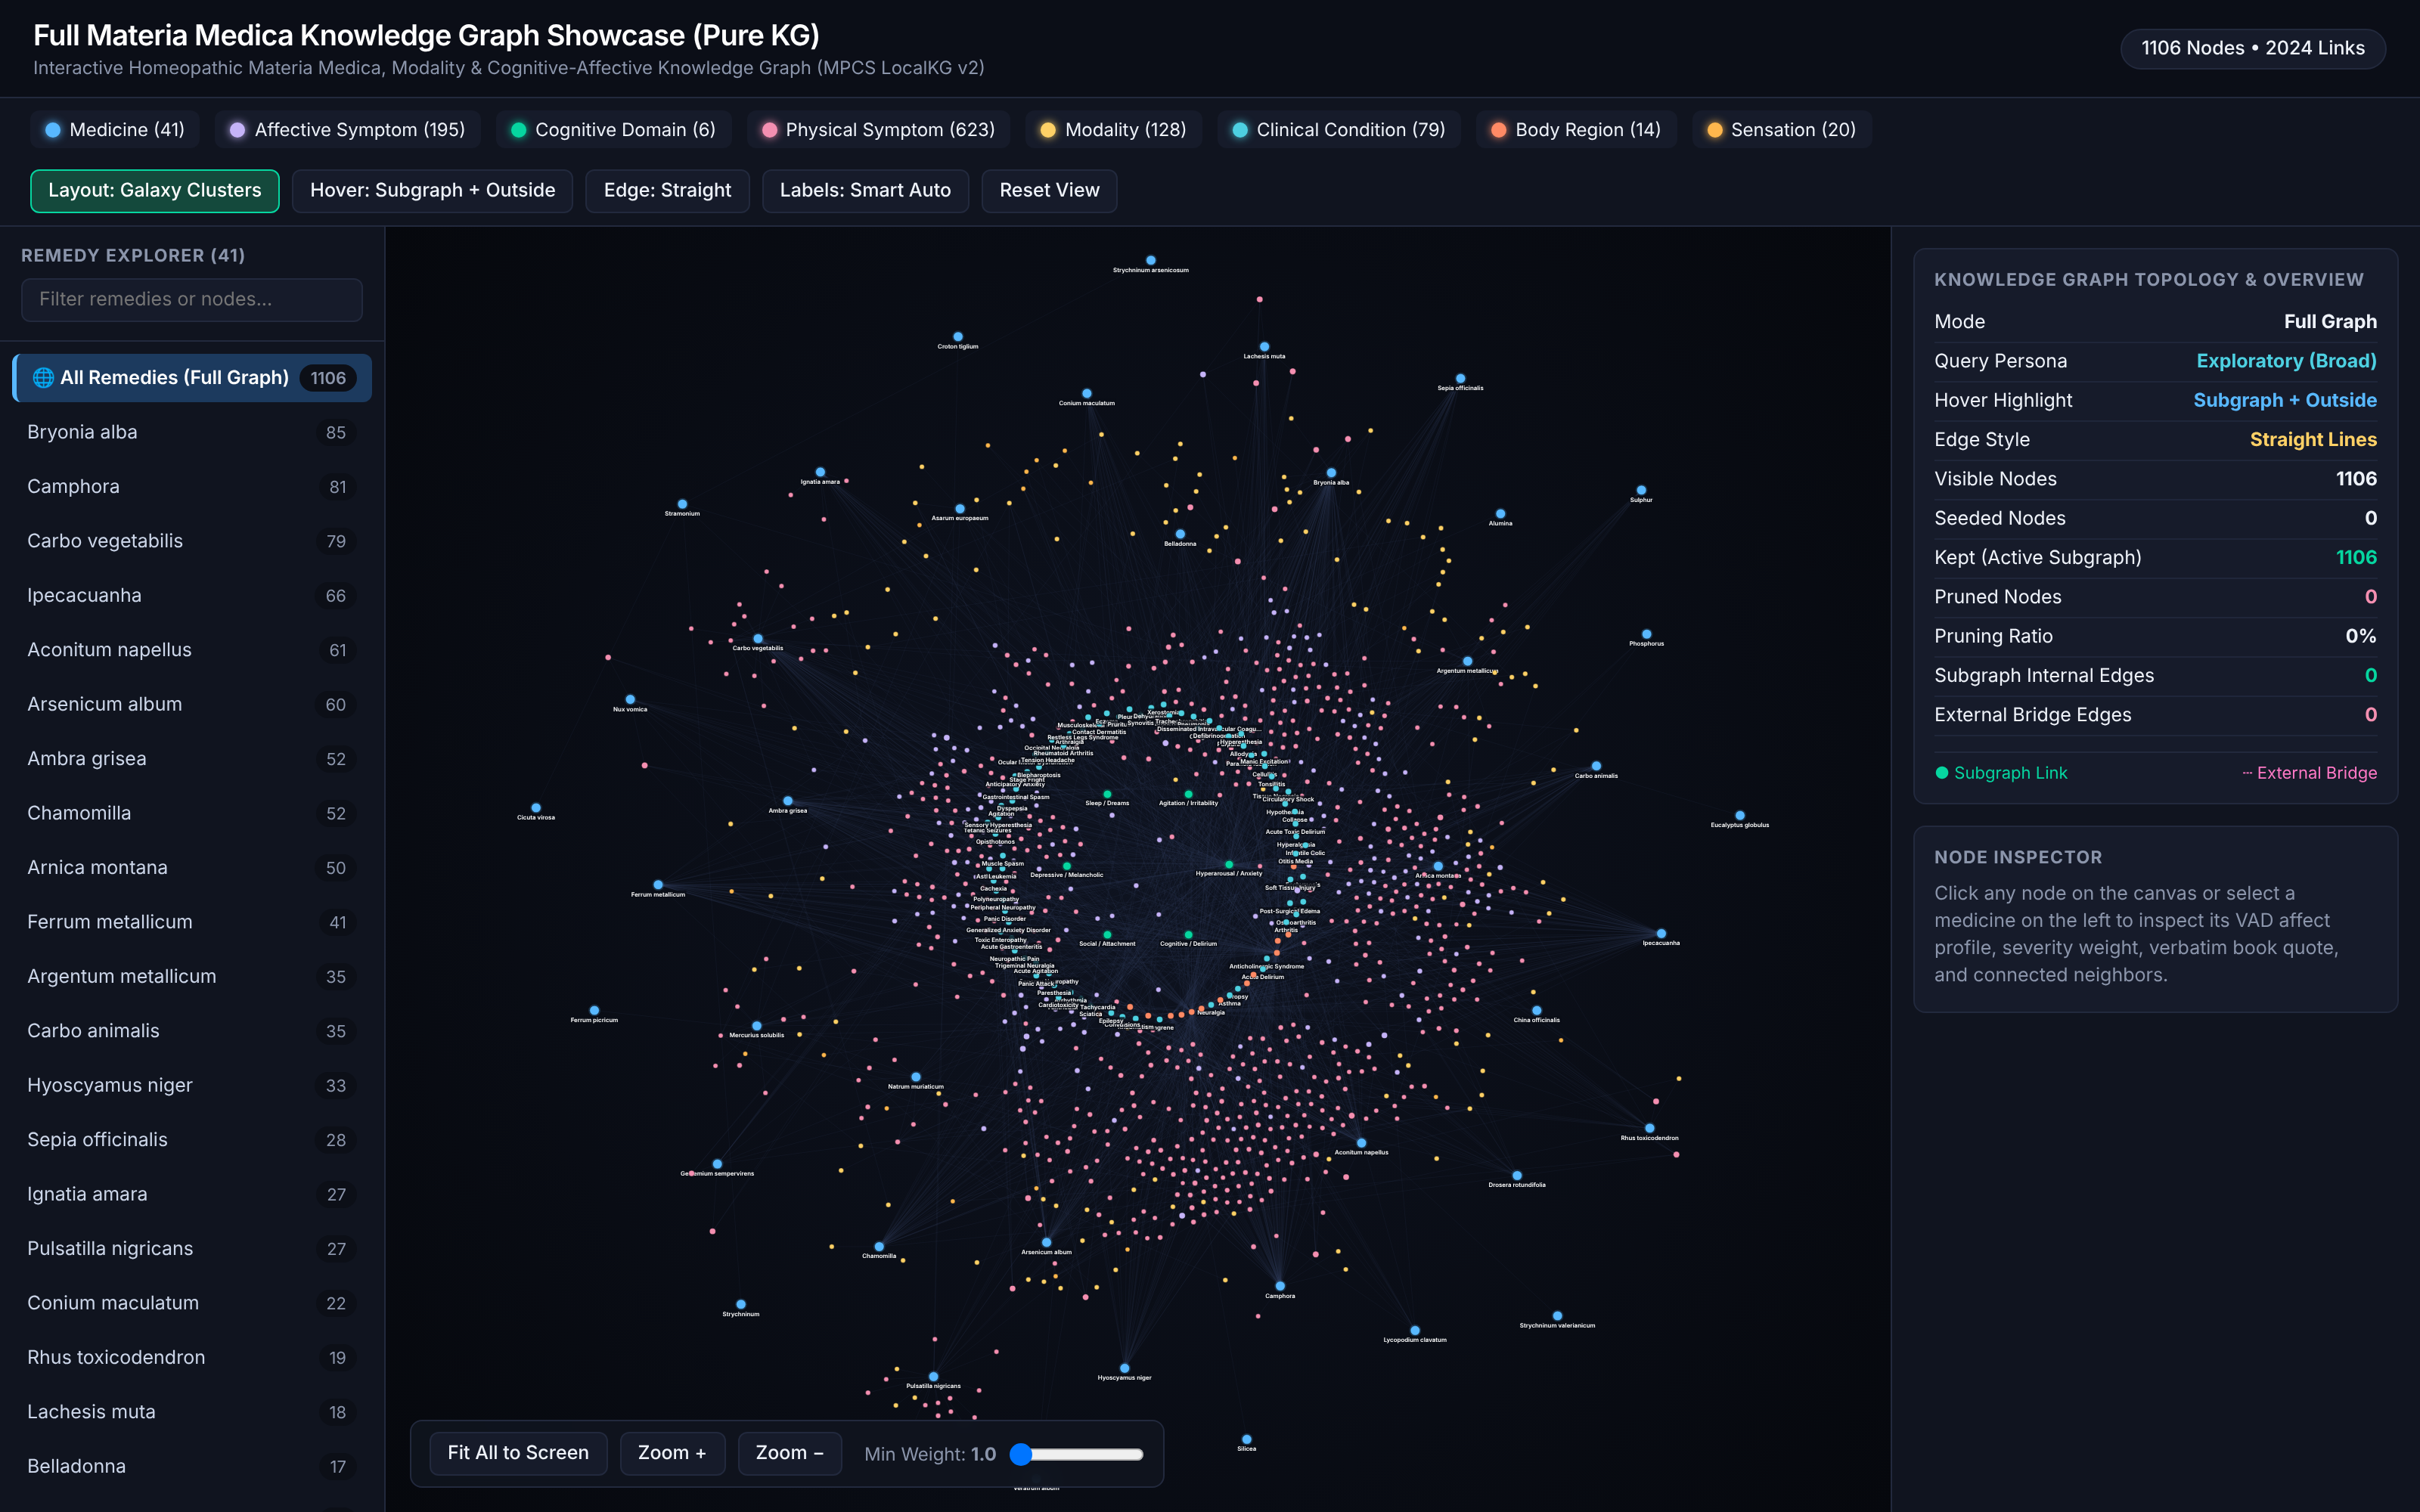
\includegraphics[width=0.85\linewidth]{figures/kg_full.png}
\caption{The complete Materia Medica graph (1,106 nodes, 2,024 edges) in the interactive viewer.}
\label{fig:kgfull}
\end{figure}

\chapter{Dual-Persona Graph Query Engine}\label{ch:persona}
% ==================================================================
The query engine (\code{LocalKG/src/lkg/query/persona\_engine.py}) answers a free-text query with a ranked subgraph. Its single most important parameter is the activation threshold that decides which nodes are returned. Two settings, called \emph{personas}, are provided.

Seeds come from an inverted index over node text (2,236 tokens), scaled by arousal and weight; energy then spreads for at most two hops over the active frontier and is normalised.

\section{Dual-Threshold Partition}
With normalised score $s(v)$, nodes are partitioned as
\begin{equation}
  \text{class}(v) = \begin{cases}
  \text{core} & s(v) \ge \theta_{\text{conf}} = 0.70,\\
  \text{exploratory} & 0.35 = \theta_{\text{expl}} \le s(v) < \theta_{\text{conf}},\\
  \text{pruned} & s(v) < \theta_{\text{expl}}.
  \end{cases}
\end{equation}
The \emph{confident} persona returns only core nodes and is meant for quick, high-precision answers. The \emph{exploratory} persona returns core and exploratory nodes, which exposes related remedies, modalities and conditions for differential comparison (Figure~\ref{fig:persona}). Edges are then classified as \emph{internal} (both ends active) or \emph{bridging} (one end active). Pruned nodes are discarded before any result objects are created, which is the main source of its speed.

\begin{figure}[H]
\centering
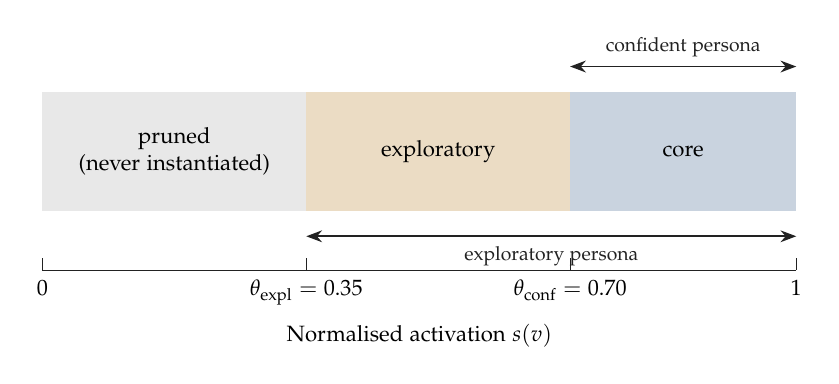
\begin{tikzpicture}
\begin{axis}[rep,height=4.6cm,width=0.92\linewidth,
  xmin=0,xmax=1,ymin=-0.2,ymax=1.2,clip=false,ytick=\empty,axis y line=none,
  xlabel={Normalised activation $s(v)$},xtick={0,0.35,0.70,1},
  xticklabels={0,$\theta_{\text{expl}}=0.35$,$\theta_{\text{conf}}=0.70$,1},ymajorgrids=false]
\fill[light!60] (axis cs:0,0.15) rectangle (axis cs:0.35,0.85);
\fill[ochrel] (axis cs:0.35,0.15) rectangle (axis cs:0.70,0.85);
\fill[navyl] (axis cs:0.70,0.15) rectangle (axis cs:1,0.85);
\node[font=\footnotesize,align=center] at (axis cs:0.175,0.5) {pruned\\(never instantiated)};
\node[font=\footnotesize,align=center] at (axis cs:0.525,0.5) {exploratory};
\node[font=\footnotesize,align=center] at (axis cs:0.85,0.5) {core};
\draw[ink,line width=0.6pt,{Stealth}-{Stealth}] (axis cs:0.70,1.0) -- node[above,font=\scriptsize]{confident persona} (axis cs:1,1.0);
\draw[ink,line width=0.6pt,{Stealth}-{Stealth}] (axis cs:0.35,0.0) -- node[below,font=\scriptsize]{exploratory persona} (axis cs:1,0.0);
\end{axis}
\end{tikzpicture}
\caption{Dual-threshold partition of graph nodes. The two personas differ only in the lower bound of the returned band.}
\label{fig:persona}
\end{figure}

% ==================================================================
\chapter{Integration of LocalKG with MPCS}\label{ch:bridge}
% ==================================================================
The bridge (\code{bridge\_engine.py}) processes one query in four stages (Figure~\ref{fig:bridge}).

\begin{enumerate}
  \item \textbf{Safety check.} A regular expression detects emergency descriptions (chest pain, difficulty breathing, severe bleeding, stroke, loss of consciousness, suicidal intent and similar). On a match, deliberation stops and the response is an \code{alert} with a referral to emergency services. In parallel the query's percept is checked against the Bloom filter.
  \item \textbf{Graph retrieval.} The query is sent to the persona engine. A ``doctor'' user maps to the exploratory persona and a ``patient'' user to the confident persona. Remedy nodes are ranked by activation and the linked symptoms are collected from internal edges.
  \item \textbf{Decision.} Words in the query that describe modifying conditions are mapped to MPCS percepts (for example ``cold'' to \code{thermal:cold}, ``motion'' to \code{contact:firm} and \code{motion:fast}, ``night'' to \code{colour:dark}). The MPCS session then runs one cognitive step and returns an action. A mean VAD vector is computed over active graph nodes, and the route is \code{DIRECT} if the top remedy scores at least 0.65 and leads the runner-up by at least 0.18, otherwise \code{SUBGRAPH}.
  \item \textbf{Evidence.} Every active node with a stored source quote is returned with its section, grade and score, so each item in the answer can be checked against the text.
\end{enumerate}
Clinician feedback (validate, mark off-target, or teach the correct action) is passed to the MPCS session through the reward and expert-teaching interfaces described in Chapter~\ref{ch:core}.

\begin{figure}[H]
\centering
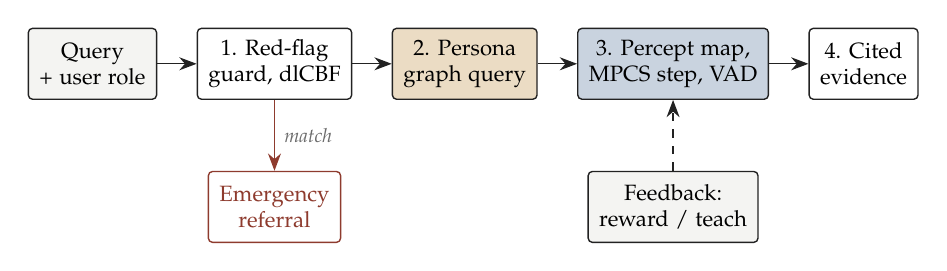
\begin{tikzpicture}[node distance=5mm and 5mm]
  \node[blkg] (q) {Query\\+ user role};
  \node[blk,right=of q] (s1) {1. Red-flag\\guard, dlCBF};
  \node[blko,right=of s1] (s2) {2. Persona\\graph query};
  \node[blkn,right=of s2] (s3) {3. Percept map,\\MPCS step, VAD};
  \node[blk,right=of s3] (s4) {4. Cited\\evidence};
  \node[blk,fill=white,below=9mm of s1,text=rust,draw=rust] (em) {Emergency\\referral};
  \node[blkg,below=9mm of s3] (fb) {Feedback:\\reward / teach};
  \draw[arr] (q)--(s1); \draw[arr] (s1)--(s2); \draw[arr] (s2)--(s3); \draw[arr] (s3)--(s4);
  \draw[arr,draw=rust] (s1)--node[lbl,right]{match}(em);
  \draw[darr] (fb)--(s3);
\end{tikzpicture}
\caption{The four stages of the bridge. An emergency match stops processing after stage 1.}
\label{fig:bridge}
\end{figure}

\chapter{Experimental Evaluation}\label{ch:results}
% ==================================================================
\section{Setup}
All MPCS experiments use Bank~v3 (700 records) with 480 clean archetype queries and 480 noisy queries in which features are perturbed. The action space has five actions. A recommendation is \emph{unsafe} if the ground truth is \code{alert} or \code{withdraw} and the system chooses \code{approach} or \code{ignore}. Memory footprint is measured by recursive traversal of all Python objects, and latency with \code{time.perf\_counter}. All schemes were run in one process by \code{LocalKG/experiments/benchmark\_indexing\_and\_tide.py}; raw results are in \code{docs/benchmark\_indexing\_tide.json}. Experiments ran single-threaded in CPython on a laptop CPU; absolute latencies should be compared only within a table.

\section{Indexing Schemes and MPCS Generations}
Table~\ref{tab:master} compares two classical baselines, the Bloom filter used alone, the global top-5 baseline (B2) and five MPCS generations.

\begin{table}[H]
\centering
\caption{Indexing schemes and MPCS generations on Bank~v3 (700 records, 480 clean and 480 noisy queries). Acc.\ is top-1 action accuracy; R@3 is the rate at which the correct action is among the top three.}
\label{tab:master}
\small
\setlength{\tabcolsep}{4.5pt}
\begin{tabular}{@{}lrrrrrrr@{}}
\toprule
& \multicolumn{2}{c}{Cost} & \multicolumn{3}{c}{Clean} & \multicolumn{2}{c}{Noisy}\\
\cmidrule(lr){2-3}\cmidrule(lr){4-6}\cmidrule(l){7-8}
Scheme & KB & ms & Acc. & R@3 & Unsafe & Acc. & Unsafe\\
\midrule
Exact KNN & 319.6 & 5.03 & 94.8 & 99.8 & 0.0 & 87.9 & 3.8\\
BM25 & 420.2 & 2.43 & 94.4 & 99.8 & 0.0 & 88.1 & 0.4\\
dlCBF alone & 8.8 & 0.017 & 50.2 & 67.7 & 1.2 & 29.4 & 0.4\\
\midrule
B2 Global top-5 & 981.2 & 10.49 & 79.6 & 98.8 & 0.0 & 73.3 & 1.2\\
B2 + dlCBF gate & 981.2 & 5.04 & 45.6 & 68.1 & 0.0 & 26.5 & 0.0\\
\midrule
G4 Core (per action) & 981.2 & 4.67 & 34.2 & 80.4 & 31.2 & 34.6 & 30.4\\
G5 HyST & 981.2 & 12.55 & 64.0 & 82.7 & 1.2 & 46.7 & 1.2\\
G6 HMGI & 981.1 & 14.46 & 34.2 & 80.4 & 31.2 & 34.6 & 30.4\\
G7 SHMF & 981.1 & 10.47 & \textbf{75.6} & 91.2 & 2.1 & \textbf{68.1} & 3.8\\
G8 KERL & 981.1 & 6.87 & 75.0 & 90.6 & 1.7 & 67.7 & 3.8\\
G9 TIDE & 981.1 & 6.56 & 75.0 & 90.6 & 1.7 & 67.7 & 3.8\\
\bottomrule
\end{tabular}
\end{table}

\begin{figure}[H]
\centering
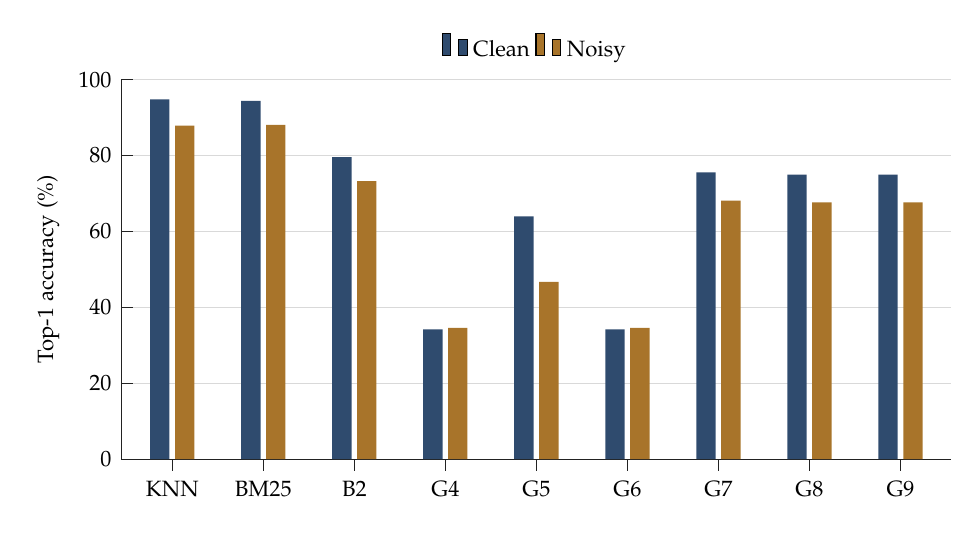
\begin{tikzpicture}
\begin{axis}[rep,ybar,bar width=7pt,height=6.4cm,
  ymin=0,ymax=100,ylabel={Top-1 accuracy (\%)},
  symbolic x coords={KNN,BM25,B2,G4,G5,G6,G7,G8,G9},xtick=data,
  enlarge x limits=0.07,legend style={at={(0.5,1.02)},anchor=south},legend columns=2]
\addplot[fill=navy,draw=none] coordinates {(KNN,94.8)(BM25,94.4)(B2,79.6)(G4,34.2)(G5,64.0)(G6,34.2)(G7,75.6)(G8,75.0)(G9,75.0)};
\addplot[fill=ochre,draw=none] coordinates {(KNN,87.9)(BM25,88.1)(B2,73.3)(G4,34.6)(G5,46.7)(G6,34.6)(G7,68.1)(G8,67.7)(G9,67.7)};
\legend{Clean,Noisy}
\end{axis}
\end{tikzpicture}

\vspace{4pt}
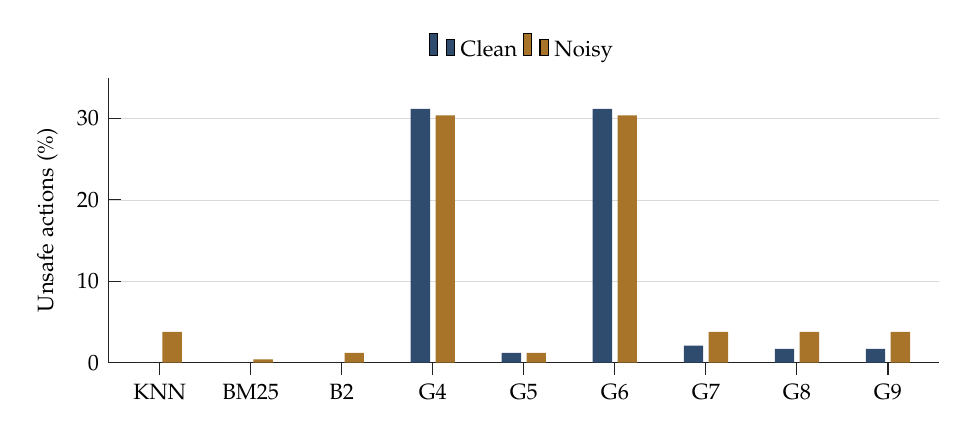
\begin{tikzpicture}
\begin{axis}[rep,ybar,bar width=7pt,height=5.2cm,
  ymin=0,ymax=35,ylabel={Unsafe actions (\%)},
  symbolic x coords={KNN,BM25,B2,G4,G5,G6,G7,G8,G9},xtick=data,
  enlarge x limits=0.07,legend style={at={(0.5,1.02)},anchor=south},legend columns=2]
\addplot[fill=navy,draw=none] coordinates {(KNN,0.0)(BM25,0.0)(B2,0.0)(G4,31.2)(G5,1.2)(G6,31.2)(G7,2.1)(G8,1.7)(G9,1.7)};
\addplot[fill=ochre,draw=none] coordinates {(KNN,3.8)(BM25,0.4)(B2,1.2)(G4,30.4)(G5,1.2)(G6,30.4)(G7,3.8)(G8,3.8)(G9,3.8)};
\legend{Clean,Noisy}
\end{axis}
\end{tikzpicture}
\caption{Accuracy (top) and unsafe-action rate (bottom) for the baselines and MPCS generations. Hard-slot filtering (G5 onwards) removes almost all unsafe actions of the per-action engine (G4).}
\label{fig:acc}
\end{figure}

\noindent The main observations are:
\begin{itemize}
  \item \textbf{Classical baselines are strong on this data.} Exact KNN and BM25 reach about 94\% clean accuracy because Bank~v3 queries are close to stored archetypes. They are included as an upper reference; they provide no reward learning, no reflexes and no evidence routing.
  \item \textbf{Per-action voting fails without hard constraints.} G4 scores each action from its own top-5 memories. Weakly related, high-reward memories of an incompatible action can then outvote exact matches, giving 34.2\% accuracy and 31.2\% unsafe actions. The global top-5 baseline (B2) does not have this failure.
  \item \textbf{Hard slots fix safety.} G5 HyST reduces unsafe actions from 31.2\% to 1.2\% (a 26-fold reduction) and raises clean accuracy to 64.0\%.
  \item \textbf{Relaxation recovers coverage.} HyST alone leaves 18.3\% of clean queries with no candidates. SHMF retries with relaxed constraints, raising clean accuracy to 75.6\% and noisy accuracy to 68.1\%, at the cost of a small rise in unsafe actions (2.1\% clean, 3.8\% noisy).
  \item \textbf{KERL and TIDE trade 0.6 points of accuracy for safety and explanation.} The near-miss guard lowers clean unsafe actions to 1.7\% and adds evidence routing, and both are faster than SHMF because the guard shrinks the set that is scored.
  \item \textbf{The Bloom filter is not a retrieval method.} Used as a hard gate it blocks most perturbed queries; used as a hint it costs 0.017\ms{} and 8.8\,KB.
\end{itemize}

\section{TIDE Anytime Budgets}
Table~\ref{tab:tide} reports TIDE under the \code{urgent} flag with candidate budgets from 3 to the full candidate set.

\begin{table}[H]
\centering
\caption{TIDE under the urgent flag. ``Read'' is the mean number of candidates read out of those available. ``Agree'' is the agreement of the fast decision with the passive full read. The unsafe rate is 1.2\% in every row.}
\label{tab:tide}
\small
\begin{tabular}{@{}l rrrr rrr@{}}
\toprule
& \multicolumn{4}{c}{Clean} & \multicolumn{3}{c}{Noisy}\\
\cmidrule(lr){2-5}\cmidrule(l){6-8}
Budget & Read & ms & Acc. & Agree & Read & Acc. & Agree\\
\midrule
$B=3$ & 2.2 / 25.4 & 3.47 & \textbf{71.9} & 73.2 & 1.6 / 19.0 & \textbf{50.8} & 80.3\\
$B=5$ & 3.3 / 25.4 & 3.45 & 70.6 & 71.8 & 2.5 / 19.0 & 49.6 & 77.2\\
$B=10$ & 5.6 / 25.4 & 4.37 & 67.9 & 76.1 & 4.2 / 19.0 & 48.5 & 79.7\\
$B=20$ & 9.2 / 25.4 & 6.61 & 67.3 & 75.9 & 6.7 / 19.0 & 47.3 & 76.8\\
$B=50$ & 14.4 / 25.4 & 6.35 & 65.4 & 77.1 & 10.5 / 19.0 & 46.9 & 72.2\\
Full & 25.4 / 25.4 & 4.71 & 64.8 & 100.0 & 19.0 / 19.0 & 46.2 & 100.0\\
\bottomrule
\end{tabular}
\end{table}

Accuracy is highest at the smallest budget and falls steadily as more candidates are read: from 71.9\% at $B=3$ to 64.8\% with a full read on clean queries, and from 50.8\% to 46.2\% on noisy queries. Lower-ranked candidates add votes that dilute the consensus of the strongest, arousal-boosted seeds. This is consistent with the foraging account of memory search, in which leaving a patch early is optimal once marginal yield drops~\cite{hills2012}. The unsafe rate is unaffected because safety is enforced before reading begins, by the hard-slot filter. The passive full read agrees with the fast decision on 73.2\% of clean and 80.3\% of noisy queries at $B=3$; disagreements are logged on the stored episode so that they can be reviewed.

\section{Sufficiency Routing}
With the \code{urgent} flag off, TIDE routes each query according to its evidence margin (Table~\ref{tab:route}).

\begin{table}[H]
\centering
\caption{Distribution and accuracy of TIDE routes (urgent flag off).}
\label{tab:route}
\small
\begin{tabular}{@{}lrrrr@{}}
\toprule
& \multicolumn{2}{c}{Clean} & \multicolumn{2}{c}{Noisy}\\
\cmidrule(lr){2-3}\cmidrule(l){4-5}
Route & Share & Acc. & Share & Acc.\\
\midrule
DIRECT & 7.7\% & 97.3\% & 4.2\% & 90.0\%\\
SUBGRAPH & 88.8\% & 76.1\% & 90.4\% & 69.8\%\\
UNGROUNDED & 3.5\% & 0.0\% & 5.4\% & 11.5\%\\
\bottomrule
\end{tabular}
\end{table}

\noindent Routing is well calibrated: when TIDE commits directly it is right 97.3\% of the time on clean queries, and the cases it marks as ungrounded are indeed those where it has no reliable answer. The low share of DIRECT routes shows that the margin of $0.25$ is conservative; it could be lowered if more direct answers were wanted at some cost in accuracy.

\section{Graph Query and Integrated Pipeline}
The confident persona answers a graph query in 1.43\ms{} on average and the exploratory persona in 1.95\ms{}, 2.56 and 1.87 times faster than a linear-scan baseline.
The bridge was profiled on six queries (five ordinary and one emergency) in both roles, each repeated 25 times. Mean end-to-end latency for non-emergency queries was 3.91\ms{} (median 3.90\ms{}, 95th percentile 5.41\ms{}), and the Bloom filter check took 30\us{} on average. The fraction of graph nodes pruned ranged from 92.4\% to 99.4\%. For ``burning pains better from warmth, anxious after midnight'' the top-ranked remedy was \emph{Arsenicum album}, which matches the classical description of that remedy. The emergency query was diverted at stage 1 in every repetition. The bridge test suite (\code{LocalKG/tests/test\_localrag\_mpcs\_bridge.py}) covers initialisation, both personas, emergency gating and feedback adaptation, and all five tests pass.

% ==================================================================
\chapter{Discussion}\label{ch:discussion}
% ==================================================================
\section{What the Results Show}
The central result is that safety can be enforced as a structural property of retrieval rather than learned. Once safety-relevant features are treated as exact-match constraints, the unsafe rate becomes almost independent of everything that follows: it stays at 1.2\% across all TIDE budgets and under noisy input. The remaining layers can then be tuned for accuracy and latency without reopening the safety question.

A second result is that reading less can be better. TIDE's best accuracy comes from reading about two candidates, provided that they are the most strongly activated ones. This depends on the quality of the activation ordering, and therefore on the arousal-weighted seeding and the episode graph.

For graph construction, the hybrid extractor shows that a language model is most useful as an auditor of grounded candidates rather than as the sole extractor: recall is unchanged, every symptom keeps a verbatim quote, and no batch can fail.

\section{Limitations}
\begin{itemize}
  \item \textbf{Synthetic episode data.} Bank~v3 is generated from archetype scenes. Classical baselines reach about 94\% on it, which indicates that it is easier than real perceptual data, and MPCS has not yet been tested on real sensor streams.
  \item \textbf{Accuracy gap to classical retrieval.} The best MPCS generation is about 19 points below exact KNN on clean queries. The gap comes mainly from per-action voting inherited from the base engine; the global top-5 variant (B2) already closes about half of it.
  \item \textbf{Small extraction gold set.} The extraction comparison uses 26 keynotes over 8 remedies. Precision is not meaningful as an absolute number because the gold set is not exhaustive.
  \item \textbf{Heuristic bridge mapping.} Modality words are mapped to percepts with a fixed table, and the bridge's routing thresholds were set by hand.
  \item \textbf{Knowledge source.} The graph encodes historical claims. Its value here is as a structured, citable test corpus, not as medical knowledge.
  \item \textbf{Latency measurements.} All timings are from single-threaded Python on one machine and vary between runs by roughly a factor of two; they indicate scale, not guarantees.
\end{itemize}

\chapter{Conclusion and Future Work}\label{ch:conclusion}
% ==================================================================
This project built and evaluated a cognitive agent whose decisions are produced by explicit, inspectable structures. MPCS perceives four modalities with per-channel confidence, reacts through reflexes, retrieves from episodic memory and adapts through reward. Its retrieval path was developed in six layers, and the evaluation showed that hard-slot filtering cuts unsafe actions by a factor of 26, that automatic relaxation recovers coverage, and that time-bounded spreading activation reaches its best accuracy after reading only a few candidates. LocalKG turned a long historical text into a typed graph of 1,106 nodes in which every symptom carries a verbatim source quote, and a hybrid extractor achieved the recall of model-based extraction with no failures. The two subsystems were joined by a bridge that answers a query, with cited evidence, in about 4\ms{}.

Future work includes:
\begin{enumerate}
  \item replacing per-action voting with global top-$k$ voting inside HyST and TIDE, to close the gap to classical retrieval;
  \item evaluating MPCS on recorded multimodal sensor data rather than synthetic archetypes;
  \item enlarging the extraction gold set and adding inter-annotator agreement;
  \item mapping LocalKG entity types to standard vocabularies such as UMLS and SNOMED CT, and applying the pipeline to a modern evidence-based corpus;
  \item learning the bridge's percept mapping and routing thresholds from feedback instead of setting them by hand;
  \item using MPCS as a constraint layer around a small local language model, where the model handles language and MPCS supplies the verified subgraph that the model is allowed to use.
\end{enumerate}

% ==================================================================
\clearpage
\begin{thebibliography}{99}
\addcontentsline{toc}{chapter}{References}
\small
\bibitem{anderson2004} J.~R. Anderson, D.~Bothell, M.~D. Byrne, S.~Douglass, C.~Lebiere and Y.~Qin. An integrated theory of the mind. \emph{Psychological Review}, 111(4):1036-1060, 2004.
\bibitem{bechara1997} A.~Bechara, H.~Damasio, D.~Tranel and A.~R. Damasio. Deciding advantageously before knowing the advantageous strategy. \emph{Science}, 275(5304):1293-1295, 1997.
\bibitem{boericke1927} W.~Boericke. \emph{Pocket Manual of Homoeopathic Materia Medica}. 9th ed., Boericke and Runyon, 1927.
\bibitem{bonomi2006} F.~Bonomi, M.~Mitzenmacher, R.~Panigrahy, S.~Singh and G.~Varghese. An improved construction for counting Bloom filters. In \emph{Proc. European Symposium on Algorithms (ESA)}, pp.~684-695, 2006.
\bibitem{charnov1976} E.~L. Charnov. Optimal foraging, the marginal value theorem. \emph{Theoretical Population Biology}, 9(2):129-136, 1976.
\bibitem{collins1975} A.~M. Collins and E.~F. Loftus. A spreading-activation theory of semantic processing. \emph{Psychological Review}, 82(6):407-428, 1975.
\bibitem{damasio1994} A.~R. Damasio. \emph{Descartes' Error: Emotion, Reason, and the Human Brain}. Putnam, 1994.
\bibitem{dasgupta2018} S.~Dasgupta, T.~C. Sheehan, C.~F. Stevens and S.~Navlakha. A neural data structure for novelty detection. \emph{Proceedings of the National Academy of Sciences}, 115(51):13093-13098, 2018.
\bibitem{gutierrez2024} B.~J. Guti\'errez, Y.~Shu, Y.~Gu, M.~Yasunaga and Y.~Su. HippoRAG: Neurobiologically inspired long-term memory for large language models. In \emph{Advances in Neural Information Processing Systems}, 2024.
\bibitem{hahnemann1880} S.~Hahnemann. \emph{Materia Medica Pura}, translated by R.~E. Dudgeon. Hahnemann Publishing Society, 1880.
\bibitem{hills2012} T.~T. Hills, M.~N. Jones and P.~M. Todd. Optimal foraging in semantic memory. \emph{Psychological Review}, 119(2):431-440, 2012.
\bibitem{ji2023hallucination} Z.~Ji, N.~Lee, R.~Frieske, T.~Yu, D.~Su, Y.~Xu, E.~Ishii, Y.~Bang, A.~Madotto and P.~Fung. Survey of hallucination in natural language generation. \emph{ACM Computing Surveys}, 55(12):1-38, 2023.
\bibitem{kahneman2011} D.~Kahneman. \emph{Thinking, Fast and Slow}. Farrar, Straus and Giroux, 2011.
\bibitem{lewis2020} P.~Lewis, E.~Perez, A.~Piktus et al. Retrieval-augmented generation for knowledge-intensive NLP tasks. In \emph{Advances in Neural Information Processing Systems}, 2020.
\bibitem{mehrabian1996} A.~Mehrabian. Pleasure-arousal-dominance: A general framework for describing and measuring individual differences in temperament. \emph{Current Psychology}, 14(4):261-292, 1996.
\bibitem{mohbat2025} F.~Mohbat and M.~J. Zaki. KERL: Knowledge-enhanced personalized recipe recommendation using large language models. In \emph{Proc. Annual Meeting of the Association for Computational Linguistics (ACL)}, 2025.
\bibitem{robertson2009} S.~Robertson and H.~Zaragoza. The probabilistic relevance framework: BM25 and beyond. \emph{Foundations and Trends in Information Retrieval}, 3(4):333-389, 2009.
\bibitem{zadeh2011} L.~A. Zadeh. A note on Z-numbers. \emph{Information Sciences}, 181(14):2923-2932, 2011.
\end{thebibliography}

% ==================================================================
\appendix
\titleformat{\chapter}[display]{\normalfont\bfseries\Large}{\large\scshape Appendix \thechapter}{6pt}{\LARGE}
\chapter{Repository Map}\label{app:repo}
\begin{table}[H]
\centering
\small
\begin{tabularx}{\linewidth}{@{}l X@{}}
\toprule
Component & Location\\
\midrule
Core engine and memory banks & \code{Model/experimental/02\_core/mpcs\_engine.py}, \code{mpcs\_preset\_v2.py}, \code{mpcs\_preset\_v3.py}\\
HyST & \code{Model/experimental/04\_hyst/hyst\_layer.py}\\
HMGI & \code{Model/experimental/05\_hmgi/hmgi\_layer.py}\\
SHMF & \code{Model/experimental/06\_shmf/shmf\_layer.py}\\
KERL & \code{Model/experimental/07\_kerl/kerl\_layer.py}\\
TIDE & \code{Model/experimental/08\_tide/tide\_layer.py}\\
Bridge and interface & \code{Model/experimental/09\_localrag\_bridge/}, \code{serve\_localrag\_mpcs\_ui.py}\\
Ontology and schemas & \code{LocalKG/src/lkg/schema/}\\
Cleaning, affect, weighting & \code{LocalKG/src/lkg/extract/affect.py}\\
Query engine & \code{LocalKG/src/lkg/query/persona\_engine.py}\\
Extraction comparison & \code{Extraction\_KRAG/homeopathy-kg/}\\
Benchmarks & \code{LocalKG/experiments/benchmark\_indexing\_and\_tide.py}, \code{benchmark\_persona\_engine.py}\\
Benchmark results & \code{docs/benchmark\_indexing\_tide.json}, \code{docs/BENCHMARK\_INDEXING\_TIDE.md}\\
Tests & \code{LocalKG/tests/}\\
\bottomrule
\end{tabularx}
\end{table}

\noindent To reproduce the main results:
\begin{lstlisting}[language=bash]
python LocalKG/experiments/benchmark_indexing_and_tide.py
python LocalKG/experiments/benchmark_persona_engine.py
python LocalKG/tests/test_localrag_mpcs_bridge.py
\end{lstlisting}

\end{document}
